\documentclass[12pt]{article}  % default square logo

\usepackage[margin=2.8cm]{geometry}
\usepackage{setspace}
\usepackage{mathptmx} % Times font
\usepackage{mathrsfs} % mathrsfs font
\usepackage{amsthm}   % theorems, definitions, lemmas

\usepackage{amsmath}  % \text{}
\usepackage[utf8]{inputenc}
\usepackage{graphicx}
\usepackage{framed} % frames
\usepackage{hyperref}
\usepackage{amssymb}  % empty set
\usepackage{multicol} % multi-column
\usepackage{tabu} % advanced table layout
\usepackage{chngcntr} % figure numbering per chapter
\usepackage{lib/bcprules} % typeset inference rule

% figure numbering
\counterwithin{figure}{section}

% code listing
\usepackage{listings}
\usepackage[table]{xcolor}

% packages for drawing
\usepackage{tikz}
\usetikzlibrary{graphs}     % create graphs
\usetikzlibrary{arrows}
\usetikzlibrary{trees}

%% set code styles

\definecolor{dkgreen}{rgb}{0,0.6,0}
\definecolor{gray}{rgb}{0.5,0.5,0.5}
\definecolor{shade}{rgb}{0.8,0.8,0.8}
\definecolor{mauve}{rgb}{0.58,0,0.82}

\lstset{
  % frame=tb,
  language=scala,
  aboveskip=3mm,
  belowskip=3mm,
  showstringspaces=false,
  columns=flexible,
  basicstyle={\small\ttfamily},
  numbers=none,
  numberstyle=\tiny\color{gray},
  keywordstyle=\color{blue},
  commentstyle=\color{dkgreen},
  stringstyle=\color{mauve},
  breaklines=true,
  breakatwhitespace=true,
  tabsize=3,
  xleftmargin=\parindent
}

% definitions, theorems

\theoremstyle{remark}
\newtheorem*{definition}{\textsc{Definition}}
\newtheorem*{theorem}{\textsc{Theorem}}
\newtheorem*{lemma}{\textsc{Lemma}}

\onehalfspacing

%end the preamble and start the document
\begin{document}

\begin{titlepage}

  \begin{center}

    %% \vspace{20cm}
    \vspace*{2\baselineskip}
    % Title
    {\LARGE A Study of Capability-Based Effect Systems\\[2cm] }

    % Author and supervisor
    \noindent
    {\large Fengyun Liu} \\[2cm]

    \noindent
    \emph{A thesis submitted for the degree of Master of Computer
      Science \\
    at École Polytechnique Fédérale de Lausanne} \\[1.8cm]

    \textit{Supervisors}

    \noindent
    \begin{multicols}{3}
    % Supervisor \\
    {\large Martin Odersky} \\
    Professor \\
    \vfill
    \columnbreak
    % Mentor \\
    {\large Nada Amin} \\
    PhD Student \\
    \vfill
    \columnbreak
    % Mentor \\
    {\large Sandro Stucki}\\
    PhD Student \\
    \end{multicols}

    \vspace*{2\baselineskip}

    \noindent
    {School of Computer and Communication Sciences \\[1cm]}
    % Upper part of the page. The '~' is needed because \\
    % only works if a paragraph has started.
    \includegraphics[width=0.5\textwidth]{img/epfl}~\\[1cm]
    \noindent
    Lausanne, January 2016 \\[1cm]

    %\vfill

    % Bottom of the page
    %% {\large \today}

  \end{center}

\end{titlepage}

%% \include{content/dedication}        % include a dedication.tex file
%% \include{content/acknowlegements}   % include an acknowledgements.tex file
\section*{\centering Abstract}
\addcontentsline{toc}{section}{Abstract}

The problem of \emph{effect polymorphism} is the main obstacle to the
wide adoption of effect systems in the programming community. The
absence of effect systems reduces compiler optimization opportunities
and deprives programmers of the freedom to impose effect constraints
on APIs in parallel and distributed computations.

This study shows that \emph{capability-based} effect systems, equipped
with \emph{stoic functions} and \emph{free functions}, can easily
solve the problem of \emph{effect polymorphism} without incurring
notational burden on programmers. This advantage makes
capability-based effect systems stand a better chance to be adopted by
the programming community.

The central idea of \emph{capability-based} effect system is that an
instance of capability is required in order to make side effects. If
capabilities are passed as function parameters, by tracking
capabilities in the type system we can track effects in the program.

To ensure that capabilities are passed through function parameters,
instead of being captured from the environment, we need to impose a
\emph{variable-capturing discipline}, stipulating that capability
variables cannot be captured. Functions observe the discipline are
called \emph{stoic functions}, while functions don't observe the
discipline are called \emph{free functions}.
          % include the abstract

\tableofcontents            % generate and include a table of contents
% \listoffigures              % generate and include a list of figures

%now include the files of latex for each of the chapters etc
\section{Introduction}

The objective of this study is to explore the theoretical foundations
as well as conceptual possibilities of capability-based effect
systems. In this chapter, we'll discuss the motivation, the core ideas
and contributions of this study.

\subsection{Motivation}

The main motivation is to turn Scala into an effect-disciplined
programming language. Currently, Scala doesn't have the ability to
track effects in the type system. This poses a problem in distributed
and parallel programming. For example, in parallel computing, there's
often the need to stipulate that the functions passed to \emph{pmap}
have no side effects.

\begin{lstlisting}[language=Scala]
def pmap(xs: List[Int], f: Int => Int): List[Int]
\end{lstlisting}

However, currently it's impossible for the library author to impose
the constraint in the type system. A central problem in introducing an
effect system in Scala is how to handle the problem of \emph{effect
  polymoprhism}.

The problem of \emph{effect polymorphism} can be illustrated by the
\emph{map} function:

\begin{lstlisting}[language=Scala]
  def map[A,B](f: A => B)(l: List[A]) = l match {
    case Nil => Nil
    case x::xs => f(x)::map(f)(l)
  }
\end{lstlisting}

In an effect system, the effect of \emph{map} depends on the passed in
function \emph{f}. If \emph{f} has IO effects, then \emph{map} also
has IO effects. If \emph{f} is pure, then \emph{map} is pure as
well.

A type-and-effect system has been proposed for
Scala\cite{lukas2014effect}. The proposed type-and-effect system
requires programmers to annotate the function \emph{map} as follows:

\begin{lstlisting}[language=Scala]
def map[A, B](f: A -> B)(l: List[A]): List[B] @pure(f)
\end{lstlisting}

The annotation says that the effect of \emph{map} depends on the
function \emph{f}.  Though this work has made some improvements in
handling \emph{effect polymorphism} compared to previous
type-and-effect systems, it still incurs some notational burden on
programmers. The system is not well received in the Scala community,
mainly due to its notational verbosity in handling \emph{effect
  polymorphism}

Monad-based effect systems have a success in Haskell. However, as we
will see, monad-based effect systems only work in lazy evaluation
languages, which is not a good fit for Scala because Scala is
strict. On the other hand, monad-based effect systems also face the
problem of \emph{effect polymorphism}. As reported in Chapter 1
section 6 of the thesis\cite{lippmeier2009type}, almost every general
purpose higher-order function in Haskell needs both a monadic version
and non-monadic version. For example, following code snippet shows the
signature for two versions of the \emph{map} function. The duplication
of code is a pity for programmers.

\begin{lstlisting}[language=Haskell]
  map :: (a -> b) -> List a -> List b
  mapIO :: (a -> IO b) -> List a -> IO (List b)
\end{lstlisting}

Given this situation, we are compelled to find a new approach to the
effect polymorphism problem, and \emph{capability-based} effect
systems seem to be a promising direction.

\subsection{Capability-based Effect Systems}

The central idea of \emph{capability-based} effect system is that an
instance of capability is required in order to make side effects. If
capabilities are passed as function parameters, by tracking
capabilities in the type system we can track effects in the program.

To ensure that capabilities are passed through function parameters,
instead of being captured from the environment, we need to impose a
\emph{variable-capturing discipline}, stipulating that capability
variables cannot be captured. Functions observe the discipline are
called \emph{stoic functions}, while functions don't oberve the
discipline are called \emph{free functions}.

With the combination of free functions and stoic functions,
\emph{capability-based} effect systems can solve the problem of
\emph{effect polymorphism} easily, while incurring no syntactical
burden. For example, instead of having two versions of \emph{map},
following \emph{map} is effect polymorphic.

\begin{lstlisting}[language=Scala]
  def map[A,B](f: A => B)(l: List[A]) = l match {
    case Nil => Nil
    case x::xs => f(x)::map(f)(l)
  }
\end{lstlisting}

When the passed function \emph{f} is pure, \emph{map} is pure as
well. In contrast, if \emph{f} is impure, then \emph{map} is also
impure. No additional annotation is required for effect polymorphism
to work. We'll see details of effect polymorphism in system
STLC-Impure.

\subsection{Contributions}

The main contributions of this study are as follows:

\begin{itemize}
\item Formulated and proved soundness and effect safety of four
  capability-based effect systems, which can serve as the fundation
  for implementing capability-based effect system in functional
  programming languages. The formalization is done in Coq based on the
  locally-nameless representation\cite{chargueraud-11-ln} and hosted
  on github\footnote{\url{https://github.com/liufengyun/stoic}}.
\item Proposed an approach to solve the problem of \emph{effect
    polymorphism} in capability-based effect systems with both free
  functions and stoic functions. The solution is much simpler and more
  elegant than in type-and-effect systems and monad-based effect
  systems.
\end{itemize}

\subsection{Structure of Report}

In following chapters, we'll introduce four systems of increasing
complexity, namely STLC-Pure, F-Pure, STLC-Impure and F-Impure.

\begin{itemize}
\item STLC-Pure is an variant of STLC with only stoic functions.
\item STLC-Impure is an extension of STLC-Pure with free functions and subtyping.
\item F-Pure is an extension of STLC-Pure with universal types.
\item F-Impure is an extension of F-Pure with free functions.
\end{itemize}

\section{Simply Typed Lambda Calculus - Pure}

This chapter describes a variant of the \emph{simply typed
  lambda-calculus} with the exension of capabilities. We call this
system \emph{STLC Pure}, because in this system all functions must
observe a variable-capturing discipline.  In later chapters, we'll see
the development of impure systems where there are both
effect-disciplined functions which observe the variable-capturing
discipline, and ordinary functions which don't observe the
variable-capturing discipline.

The system STLC Pure, though conceptually simple, can quite well
demonstrate the core idea of capability-based type-and-effect
systems. We'll first introduce the formalization, then discuss
soundness and effect safety. Concepts introduced here will be a
foundation for more complex systems in later chapters.

\subsection{Definitions}

Formally, STLC Pure is obtained by introducing capability type and
imposing variable capability-capturing discipline on lambda
abstractions.  Figure~\ref{fig:stlc-pure-definition} presents the full
definition of STLC Pure.

The syntax is almost the same as standard STLC, except the addition of
capability type \emph{E} and addition of variables as values. The
evaluation rules are exactly the same, with standard call-by-value
small-step semantics. The typing rule T-Abs is slightly changed by
performing an operation on the environment. The peculiarities in the
formalization are explained below.

\begin{figure}[ht]
\begin{framed}
\begin{multicols}{2}

\textbf{Syntax}

\begin{tabu} to \linewidth {l l l X[r]}
  t   & ::= &                    & terms:               \\
      &     &  x                 & variable             \\
      &     & $\lambda$ x:T.t    & abstraction          \\
      &     & t t                & application          \\
\\
  v   & ::= &                    & values:              \\
      &     & $\lambda$ x:T.t    & abstraction value    \\
      &     & x                  & variable value       \\
\\
  T   & ::= &                    & types:               \\
      &     & B                  & basic type           \\
      &     & E                  & capability type      \\
      &     & T $\to$ T          & type of functions    \\
\end{tabu}

\hfill\\

\textbf{Evaluation} \hfill \framebox[1.2\width][r]{$t \longrightarrow t'$}

\infrule[E-App1]
{ t_1 \longrightarrow t'_1 }
{ t_1 \; t_2 \longrightarrow t'_1 \; t_2 }

\infrule[E-App2]
{ t_2 \longrightarrow t'_2 }
{ v_1 \; t_2 \longrightarrow v_1 \; t'_2 }

\infax[E-AppAbs]
{ (\lambda x:T.t_1) v_2 \longrightarrow [x \mapsto v_2]t_1 }

\columnbreak

\textbf{Typing}  \hfill \framebox[1.2\width][r]{$\Gamma \vdash x : T$}

\infrule[T-Var]
{ x: T \in \Gamma }
{ \Gamma \vdash x : T }

\infrule[T-Abs]
{ pure(\Gamma),\; x: S \vdash t_2 : T }
{ \Gamma \vdash \lambda x:S.t_2 : S \to T }

\infrule[T-App]
{ \Gamma \vdash t_1 : S \to T \andalso \Gamma \vdash t_2 : S }
{ \Gamma \vdash t_1 \; t_2 : T }

\textbf{Pure Environment}

\begin{center}
\begin{tabular}{l c l}
pure($\varnothing$)             & = &   $\varnothing$ \\
pure($\Gamma$, x: E)            & = &  pure($\Gamma$) \\
pure($\Gamma$, x: T)  & = &  pure($\Gamma$), x: T     \\
\end{tabular}
\end{center}

\hfill\\

\end{multicols}
\end{framed}

\caption{System STLC Pure}
\label{fig:stlc-pure-definition}
\end{figure}

\subsubsection{Variable-Capturing Discipline}

The most important change compared to standard STLC lies in following
typing rule:

\infrule[T-Abs]
{ pure(\Gamma) , x: S \vdash t_2 : T }
{ \Gamma \vdash \lambda x:S.t_2 : S \to T }

This typing rule imposes a \emph{variable-capturing discipline} on
lambda abstractions. This discipline stipulates that only variables
whose type is not a capability type can be captured in a lambda
abstraction.

The discipline is implemented with the helper function \emph{pure},
which removes any variable bindings of the capability type \emph{E}
from the typing environment. It's easy to verify the \emph{pure}
function satisfies following properties:

\begin{lemma}[Pure-Distributivity]
  pure (E, F) = pure E, pure F
\end{lemma}

\begin{lemma}[Pure-Idempotency]
  pure (pure E) = pure E
\end{lemma}

\subsubsection{Stoic Functions}

The variable-capturing discipline makes the functions in STLC Pure
essentially different from functions in standard STLC. In STLC,
functions can capture any variables in scope, while in STLC Pure
functions can only capture variables whose type is not a capability
type($E$). To differentiate them (which is important as in later
systems both exist), we call the more effect-disciplined functions as
\emph{stoic functions}.

Stoic functions are essential in capability-based type-and-effect
systems. If functions are allowed to capture capability variables in
scope, it will be impossible to tell whether a function has side
effect or not (and what kind of effect) by just checking its
type. Stoic functions are effect-disciplined in the sense that the
only way for stoic functions to have side effects is to pass a
capability as parameter, thus it can be captured by the type system.

It's important to note that stoic functions are not necessarily pure
functions. Stoic functions can have side effects, and if they do have
side effects they are honest about that in their type signature. For
example, following function \emph{hello} is a stoic function which has
IO effects\footnote{For readability, we'll use a syntax similar to
  Scala. However, we'll use $\to$ to annotate the type of stoic
  functions, and $\Rightarrow$ for ordinary functions.}.

\begin{lstlisting}[language=Scala]
  def hello(c:IO) = println("hello, world!", c)
\end{lstlisting}

In the following code snippet, we can be sure that the function
\emph{f} is pure, as it doesn't take any capability as parameter. In
the definition of \emph{f}, it's impossible to call functions to
create side effects, as in STLC Pure all functions that can have side
effects take some capability as parameter.

\begin{lstlisting}[language=Scala]
  def twice(f: Int -> Int)(x: Int) = f (f x)
\end{lstlisting}

\subsubsection{Where do Effects Come From}

Careful readers might have noticed that in current type-and-effect system,
there is no formalization of effects. Indeed, that's an intentional
design choice. As the primary concern of this study is IO effects, we
assume the existence of primitive functions like \emph{println}, which
take capability parameters to create side effects.

\subsubsection{Where do Capabilities Come From}

In current system it is impossible to create capabilities. Where do
capabilities come from?  There are two possible answers. The first one
is that all capabilities are from the runtime and passed to the
program through the \emph{main} method.

The second one is that there are no capabilities. Capabilities can be
erased before evaluation in principle, without affecting meaning of
the program. However, in this study we only state this observation
informally and leave the formal proof to future studies.

\subsubsection{Why Treat Variables as Values}

As discussed above, in current system, there is no way to create
capabilities. It means that a function taking a capability parameter
can never be called. A soundness proof for such a system is not very
convincing. Instead, if we treat variables as values, functions that
takes a capability parameter can be called with a capability
variable. This makes the preservation proof (see below) more
convincing.

Adding variables as values doesn't break soundness or effect safety of
the system. In fact, by adding variables as values, we only added 5
lines of code in our soundness proof, and effect safety proof remains
the same.

\subsection{Soundness}

We follow the standard formulation of soundness in TAPL
\cite{pierce2002types}, which consists of \emph{progress} and
\emph{presevation}, defined as follows:

\begin{theorem}[Progress]
If $\varnothing \vdash t : T$, then either $t$ is a value or there is some
$t'$ with $t \longrightarrow t'$.
\end{theorem}

\begin{theorem}[Preservation]
If $\Gamma \vdash t : T$, and $t \longrightarrow t'$, then $\Gamma
\vdash t' : T$.
\end{theorem}

We proved both theorems in Coq based on the locally-nameless
representation. The proof of progress is the same as in STLC. However,
there is a significant difference in the proof of preservation In the
classic proof of preservation for STLC (as shown in TAPL), it depends
on a substitution lemma, which is formulated as follows:

\begin{lemma}[Subsitution-Classic]
If $\Gamma,\; x:S \vdash t : T$, and $\Gamma \vdash s : S$, then $\Gamma
\vdash [x \mapsto s]t : T$.
\end{lemma}

However, this substitution lemma doesn't hold in current system. For a
counter-example, let's assume that $\Gamma = \{f: E \to B,\;
  c:E\}$, then it's obviously that following two propositions hold:

\begin{itemize}
\item $\{f: E \to B,\; c:E\},\; x:B \vdash \lambda z:B.\,x \; : \; B \to B$.
\item $\{f: E \to B,\; c:E\},\; x:B \vdash f \; c \; : \; B$.
\end{itemize}

However, following typing relationship doesn't hold if we replace
$x$ with $f \; c$.

\begin{center}
$\{f: E \to B,\; c:E\} \vdash \lambda z:B.\,f \; c \; : \; B \to B$.
\end{center}

In fact, the substituted term $\lambda z:B.\,f \; c$ cannot be typed,
as according to the typing rules, it cannot capture the capability
variable $c$ in the environment. To overcome this problem, we
stipulate that the term $s$ to be substituted must be a
value. Remember that in current system, both lambda abstractions and
variables are values, thus subsitution of capability variables can
also happen. The new formulation is as follows:

\begin{lemma}[Subsitution-New]
  If $\Gamma,\; x:S \vdash t : T$, s is a value and
  $\Gamma \vdash s : S$, then $\Gamma \vdash [x \mapsto s]t : T$.
\end{lemma}

\subsection{Effect Safety}



\subsection{Discussion}

extensions and practicality

\section{System STLC-Impure}

This chapter describes an extension of system STLC-Pure, where there
exists both effect-disciplined functions (stoic functions) and
effect-arbitrary functions (libertine functions). As there's a
subtyping between the two kinds of functions, it's natural to
integrate subtyping in the system.

We'll first introduce the formalization, then discuss soundness and
effect safety. In the discussion, we'll focus on its difference from
system STLC-Pure.

\subsection{Definitions}

Initially, we arrived at a formualtion of the system shown in
Figure~\ref{fig:stlc-impure-definition-first}. It's a straight-forward
extension of SLTC-Pure with subtyping and libertine functions. Note
that in this formulation, we need to change the definition of the
\emph{pure} function to exclude libertine function types in the pure
environment. This restriction is important, because we're not sure
what side effects there might be inside libertine functions. If we
allow stoic functions have access to libertine functions, we'll loose
the ability to track the effects of stoic functions in the type
system.

The definition is all good, except that perservation breaks! The
problem is caused by using an impure term as \emph{Top}. To see a
concrete example, let's assume $\Gamma = \{c:E\}$. It's obvious that
following term is well-typed under $\Gamma$ as $B \to Top$:

\begin{center}
  $(\lambda x:Top. \; \lambda y:B. \; x) \; c$
\end{center}

However, after one evaluation step\footnote{Note that variables are
  values, thus we can take a step here. We can also construct a
  counter-example by wrap $c$ in a lambda abstraction like
  $\lambda x:B. c$.}, we get the term $\lambda y:B. \; c$, which can
at best be typed as $B \Rightarrow Top$. Thus preservation doesn't
hold in current formulation. This problem leads us to two different
formuations.

\begin{figure}
\begin{framed}

% multi-column separator
\setlength{\columnseprule}{0.4pt}
\begin{multicols}{2}

\textbf{Syntax}

\begin{tabu} to \linewidth {l l l X[r]}
  t   & ::= &                    & terms:               \\
      &     &  x                 & variable             \\
      &     & $\lambda$ x:T.t    & abstraction          \\
      &     & t t                & application          \\
\\
  v   & ::= &                    & values:              \\
      &     & $\lambda$ x:T.t    & abstraction value    \\
      &     & x                  & variable value       \\
\\
  T   & ::= &                    & types:               \\
      &     & \colorbox{shade}{Top}  & Top type             \\
      &     & B                  & basic type           \\
      &     & E                  & capability type      \\
      &     & T $\to$ T          & type of stoics       \\
      &     & \colorbox{shade}{T $\Rightarrow$ T} & type of libertines   \\
\end{tabu}

\hfill\\

\textbf{Evaluation} \hfill \framebox[1.2\width][r]{$t \longrightarrow t'$}

\infrule[E-App1]
{ t_1 \longrightarrow t'_1 }
{ t_1 \; t_2 \longrightarrow t'_1 \; t_2 }

\infrule[E-App2]
{ t_2 \longrightarrow t'_2 }
{ v_1 \; t_2 \longrightarrow v_1 \; t'_2 }

\infax[E-AppAbs]
{ (\lambda x:T.t_1) v_2 \longrightarrow [x \mapsto v_2]t_1 }

\textbf{Pure Environment}

\begin{center}
\begin{tabular}{l c l}
pure($\varnothing$)                   & = &   $\varnothing$ \\
pure($\Gamma$, x: E)                  & = &  pure($\Gamma$) \\
\rowcolor{gray!40}
pure($\Gamma$, x: S $\Rightarrow$ T)  & = &  pure($\Gamma$) \\
pure($\Gamma$, x: T)                  & = &  pure($\Gamma$), x: T     \\
\end{tabular}
\end{center}

\columnbreak

\textbf{Typing}  \hfill \framebox[1.2\width][r]{$\Gamma \vdash x : T$}

\infrule[T-Var]
{ x: T \in \Gamma }
{ \Gamma \vdash x : T }

\infrule[T-Abs1]
{ pure(\Gamma),\; x: S \vdash t_2 : T }
{ \Gamma \vdash \lambda x:S.t_2 : S \to T }

\infrule[T-Abs2]
{  \colorbox{shade}{$\Gamma,\; x: S \vdash t_2 : T$} }
{  \colorbox{shade}{$\Gamma \vdash \lambda x:S.t_2 : S \Rightarrow T$} }

\infrule[T-App]
{ \Gamma \vdash t_1 : S \to T \andalso \Gamma \vdash t_2 : S }
{ \Gamma \vdash t_1 \; t_2 : T }

\infrule[T-Sub]
{  \colorbox{shade}{$\Gamma \vdash t : S \andalso S <: T$} }
{  \colorbox{shade}{$\Gamma \vdash t : T$} }

\colorbox{shade}{\textbf{Subtyping}}  \hfill \framebox[1.2\width][r]{$S <: T$}

\infax[S-Top]{ T <: Top }

\infax[S-Refl]{ T <: T }

\infrule[S-Trans]
{ S <: U \andalso U <: T }
{ S <: T }

\infrule[S-Degen]
{ S \to T }
{ S \Rightarrow T }

\infrule[S-Fun1]
{ S1 <: S2 \andalso T2 <: T1 }
{ S2 \to T2 <: S1 \to T1 }

\infrule[S-Fun2]
{ S1 <: S2 \andalso T2 <: T1 }
{ S2 \Rightarrow T2 <: S1 \Rightarrow T1 }

\hfill\\

\end{multicols}
\end{framed}

\caption{System STLC-Impure First Formulation}
\label{fig:stlc-impure-definition-first}
\end{figure}

The first one is to introduce two different Top types, one is pure and
the other is impure. The capability type E and libertine function type
$S \Rightarrow T$ are not sutype of the pure Top. The subtyping
hierarchy is shown in Figure~\ref{fig:stlc-impure-subtyping-tree}. This
formulation works well, and we've proved soundness and effect safety
for the formulation. However, we lose the simplicity in the type
system. And it's counter-intuitive to forbid Top in pure environments,
as we cannot create side effects with a variable of type Top.

\begin{figure}
\centering

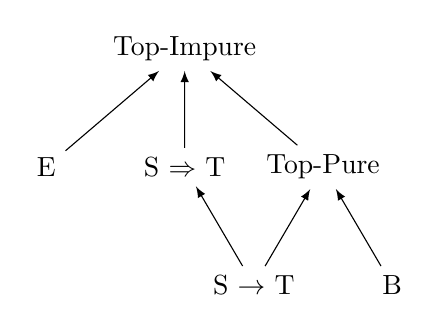
\begin{tikzpicture}[sibling distance=5em,
  every node/.style = {align=center},
  edge from parent/.style={draw,latex-}]
  \node {Top-Impure}
  child { node {E} }
  child { node (libertine) {S $\Rightarrow$ T} }
  child { node {Top-Pure}
    child { node (stoic) {S $\to$ T} }
    child { node {B} } };
  \path [draw, -latex] (stoic) -- (libertine);
\end{tikzpicture}

\caption{Subtyping: Top-Pure and Top-Impure}
\label{fig:stlc-impure-subtyping-tree}
\end{figure}

The second possibility is to keep the elegance of the type system and
changes the evaluation rules. We know that all terms of the type Top
are equivalent, because we can do nothing with a term of type Top. It
implies we can substitute them arbitrarily without changing the
meaning of the term. This observation inspires us to introduce a
\emph{top} value and change the standard E-AppAbs rule to two
evaluation rules as follows:

\infrule[E-AppAbs1]
{ T \neq Top }
{ (\lambda x:T.t_1) v_2 \longrightarrow [x \mapsto v_2]t_1 }

\infrule[E-AppAbs2]
{ T = Top }
{ (\lambda x:T.t_1) v_2 \longrightarrow [x \mapsto top]t_1 }

The two rules have the effect that if a function takes a parameter of
type Top, then when called it will drop the parameter and replace it
with the \emph{top} value. We follow this approach in the formulation
and the full definition is presented in
Figure~\ref{fig:stlc-impure-definition}.

\begin{figure}
\begin{framed}

% multi-column separator
\setlength{\columnseprule}{0.4pt}
\begin{multicols}{2}

\textbf{Syntax}

\begin{tabu} to \linewidth {l l l X[r]}
  t   & ::= &                    & terms:               \\
      &     & \colorbox{shade}{top} & top value            \\
      &     & x                  & variable             \\
      &     & $\lambda$ x:T.t    & abstraction          \\
      &     & t t                & application          \\
\\
  v   & ::= &                    & values:              \\
      &     & $\lambda$ x:T.t    & abstraction value    \\
      &     & x                  & variable value       \\
      &     & \colorbox{shade}{top}  & top value            \\
\\
  T   & ::= &                    & types:               \\
      &     & \colorbox{shade}{Top}  & Top type             \\
      &     & B                  & basic type           \\
      &     & E                  & capability type      \\
      &     & T $\to$ T          & type of stoics       \\
      &     & \colorbox{shade}{T $\Rightarrow$ T} & type of libertines   \\
\end{tabu}

% \hfill\\
\vspace{0.1em}

\textbf{Evaluation} \hfill \framebox[1.2\width][r]{$t \longrightarrow t'$}

\infrule[E-App1]
{ t_1 \longrightarrow t'_1 }
{ t_1 \; t_2 \longrightarrow t'_1 \; t_2 }

\infrule[E-App2]
{ t_2 \longrightarrow t'_2 }
{ v_1 \; t_2 \longrightarrow v_1 \; t'_2 }

\infrule[E-AppAbs1]
{ \colorbox{shade}{$T \neq Top$} }
{ \colorbox{shade}{$(\lambda x:T.t_1) \; v_2 \longrightarrow [x \mapsto v_2]t_1$} }

\infrule[E-AppAbs2]
{ \colorbox{shade}{$T = Top$} }
{ \colorbox{shade}{$(\lambda x:T.t_1) \; v_2 \longrightarrow [x \mapsto top]t_1$} }

\textbf{Pure Environment}

\begin{center}
\begin{tabular}{l c l}
pure($\varnothing$)                   & = &   $\varnothing$ \\
pure($\Gamma$, x: E)                  & = &  pure($\Gamma$) \\
\rowcolor{gray!40}
pure($\Gamma$, x: S $\Rightarrow$ T)  & = &  pure($\Gamma$) \\
pure($\Gamma$, x: T)                  & = &  pure($\Gamma$), x: T     \\
\end{tabular}
\end{center}

\columnbreak

\textbf{Typing}  \hfill \framebox[1.2\width][r]{$\Gamma \vdash x : T$}

\infax[T-Top]{ \colorbox{shade}{$\Gamma \vdash top : Top$} }

\infrule[T-Var]
{ x: T \in \Gamma }
{ \Gamma \vdash x : T }

\infrule[T-Abs1]
{ pure(\Gamma),\; x: S \vdash t_2 : T }
{ \Gamma \vdash \lambda x:S.t_2 : S \to T }

\infrule[T-Abs2]
{  \colorbox{shade}{$\Gamma,\; x: S \vdash t_2 : T$} }
{  \colorbox{shade}{$\Gamma \vdash \lambda x:S.t_2 : S \Rightarrow T$} }

\infrule[T-App]
{ \Gamma \vdash t_1 : S \to T \andalso \Gamma \vdash t_2 : S }
{ \Gamma \vdash t_1 \; t_2 : T }

\infrule[T-Sub]
{  \colorbox{shade}{$\Gamma \vdash t : S \andalso S <: T$} }
{  \colorbox{shade}{$\Gamma \vdash t : T$} }

\colorbox{shade}{\textbf{Subtyping}}  \hfill \framebox[1.2\width][r]{$S <: T$}

\infax[S-Top]{ T <: Top }

\infax[S-Refl]{ T <: T }

\infrule[S-Trans]
{ S <: U \andalso U <: T }
{ S <: T }

\infrule[S-Degen]
{ S \to T }
{ S \Rightarrow T }

\infrule[S-Fun1]
{ S1 <: S2 \andalso T2 <: T1 }
{ S2 \to T2 <: S1 \to T1 }

\infrule[S-Fun2]
{ S1 <: S2 \andalso T2 <: T1 }
{ S2 \Rightarrow T2 <: S1 \Rightarrow T1 }

\hfill\\

\end{multicols}
\end{framed}

\caption{System STLC-Impure}
\label{fig:stlc-impure-definition}
\end{figure}

\subsection{Soundness}

We proved both progress and preservation in Coq based on the
locally-nameless representation.

\begin{theorem}[Progress]
If $\varnothing \vdash t : T$, then either $t$ is a value or there is some
$t'$ with $t \longrightarrow t'$.
\end{theorem}

\begin{theorem}[Preservation]
If $\Gamma \vdash t : T$, and $t \longrightarrow t'$, then $\Gamma
\vdash t' : T$.
\end{theorem}

As you can imagine, now we need to different substitution lemmas in
the proof of perservation, corresponding to the two reduction rules.

\begin{lemma}[Subsitution-Non-Top]
  If $\Gamma,\; x:S \vdash t : T$, s is a value, $S \neq Top$ and
  $\Gamma \vdash s : S$, then $\Gamma \vdash [x \mapsto s]t : T$.
\end{lemma}

\begin{lemma}[Subsitution-Top]
  If $\Gamma,\; x:Top \vdash t : T$, then $\Gamma \vdash [x \mapsto top]t : T$.
\end{lemma}

\subsection{Effect Safety}

\subsubsection{Definition}

\subsubsection{Proof}

\section{System F-Pure}

In this chapter, we present the system \emph{F-Pure}, which is an
extension of the system STLC-Pure with universal types. In this
system, not only functions need to observe a variable-capturing
discipline, type abstractions also need to observe the same
variable-capturing discipline.

We'll first introduce the formalization, then discuss soundness and
effect safety. In the discussion, we'll focus on its difference from
the system STLC-Pure.

\begin{figure}
\begin{framed}

% multi-column separator
\setlength{\columnseprule}{0.4pt}
\begin{multicols}{2}

\textbf{Syntax}

\begin{tabu} to \linewidth {l l l X[r]}
  t   & ::= &                                      & terms:               \\
      &     &  x                                   & variable             \\
      &     & $\lambda$ x:T.t                      & abstraction          \\
      &     & t t                                  & application          \\
      &     & \colorbox{shade}{$\lambda$ X.t}      & type abstraction     \\
      &     & \colorbox{shade}{t [T]}              & type application     \\
\\
  v   & ::= &                    & values:              \\
      &     & $\lambda$ x:T.t    & abstraction value    \\
      &     & x                  & variable value       \\
      &     & \colorbox{shade}{$\lambda X.t$}    & type abstraction value  \\
\\
  T   & ::= &                       & types:               \\
      &     & \colorbox{shade}{X}   & type variable        \\
      &     & B                     & basic type           \\
      &     & E                     & capability type      \\
      &     & T $\to$ T             & type of functions    \\
      &     & \colorbox{shade}{$\forall$ X.T} & universal type       \\
\end{tabu}

\hfill\\

\textbf{Evaluation} \hfill \framebox[1.2\width][r]{$t \longrightarrow t'$}

\infrule[E-App1]
{ t_1 \longrightarrow t'_1 }
{ t_1 \; t_2 \longrightarrow t'_1 \; t_2 }

\infrule[E-App2]
{ t_2 \longrightarrow t'_2 }
{ v_1 \; t_2 \longrightarrow v_1 \; t'_2 }

\infax[E-AppAbs]
{ (\lambda x:T.t_1) v_2 \longrightarrow [x \mapsto v_2]t_1 }

\infrule[E-TApp]
{ \colorbox{shade}{$t_1 \longrightarrow t'_1$} }
{ \colorbox{shade}{$t_1 \; [T_2] \longrightarrow t'_1 \; [T_2]$} }

\infax[E-TappTabs]
{ \colorbox{shade}{$(\lambda X.t_1) [T_2] \longrightarrow [X \mapsto T_2]t_1$} }

\columnbreak

\textbf{Typing}  \hfill \framebox[1.2\width][r]{$\Gamma \vdash x : T$}

\infrule[T-Var]
{ x: T \in \Gamma }
{ \Gamma \vdash x : T }

\infrule[T-Abs]
{ pure(\Gamma),\; x: S \vdash t_2 : T }
{ \Gamma \vdash \lambda x:S.t_2 : S \to T }

\infrule[T-App]
{ \Gamma \vdash t_1 : S \to T \andalso \Gamma \vdash t_2 : S }
{ \Gamma \vdash t_1 \; t_2 : T }

\infrule[T-TAbs]
{ \colorbox{shade}{$pure(\Gamma),\; X \vdash t_2 : T$} }
{ \colorbox{shade}{$\Gamma \vdash \lambda X.t_2 : \forall X. T$} }

\infrule[T-TApp]
{ \colorbox{shade}{$\Gamma \vdash t_1 : \forall X.T \andalso T_2 \neq E$} }
{ \colorbox{shade}{$\Gamma \vdash t_1 \; [T_2] : [X \mapsto T_2]T$} }

\hfill\\

\textbf{Pure Environment}

\hfill

\begin{center}
\begin{tabular}{l c l}
pure($\varnothing$)             & = &   $\varnothing$ \\
pure($\Gamma$, x: E)            & = &  pure($\Gamma$) \\
pure($\Gamma$, x: T)  & = &  pure($\Gamma$), x: T     \\
\rowcolor{gray!40}
pure($\Gamma$, X)  & = &  pure($\Gamma$), X  \\
\end{tabular}
\end{center}


\end{multicols}
\end{framed}

\caption{System F-Pure}
\label{fig:f-pure-definition}
\end{figure}

\subsection{Definitions}

The system F-Pure extends STLC-Pure with universal
types. Figure~\ref{fig:f-pure-definition} presents the full definition
of F-Pure, with the difference from the system STLC-Pure highlighted.

The extension of syntax and evaluation rules are exactly the same as
the extension of standard STLC with universal types.  The essential
difference lies in the two new typing rules \textsc{T-TAbs} and
\textsc{T-TApp}. The typing rule \textsc{T-TAbs} stipulates that type
abstraction must observe the variable-capturing discipline.

\infrule[T-TAbs]
{ pure(\Gamma),\; X \vdash t_2 : T }
{ \Gamma \vdash \lambda X.t_2 : \forall X. T }

We made this design choice in order to allow universal types to be
present in pure environments. Otherwise, if type abstractions can
capture capability variables, application of a type abstraction could
generate a term of the capability type or have side effects. This
makes it incorrect to have universal types in pure environments, thus
renders universal types useless in the system.

The typing rule \textsc{T-TApp} requires that the type parameter
cannot be the capability type E. However, it's allowed to supply
non-inhabitable types like $B \to E$ as parameter to type abstraction.

% This restriction implies in system F-Pure polymorphism doesn't cover
% capability types.

\infrule[T-TApp]
{ \Gamma \vdash t_1 : \forall X.T \andalso T_2 \neq E }
{ \Gamma \vdash t_1 \; [T_2] : [X \mapsto T_2]T }

Without the restriction, preservation of the system breaks, as can be
seen from following term $t$, which has the type
$\forall T. T \to B \to T$:

\begin{center}
  $t = \lambda T. \; \lambda x:T. \; \lambda y:B. \; x$
\end{center}

If we allow $E$ as parameter to type application, the term $t [E]$ has
the type $E \to B \to E$. However, after one evaluation step, the term
$\lambda x:E. \; \lambda y:B. \; x$ cannot be typed anymore, as the
capability variable $x$ cannot be captured in the inner-most lambda;
thus preservation breaks.

The definition of the function \emph{pure} is changed slightly by
allowing type variables to be in the pure environment. This is
natural, as we know in the typing rule \textsc{T-TApp} that a type
variable cannot be of the capability type.

\subsection{Soundness}

We proved both progress and preservation of the system.

\begin{theorem}[Progress]
If $\varnothing \vdash t : T$, then either $t$ is a value or there is some
$t'$ with $t \longrightarrow t'$.
\end{theorem}

\begin{theorem}[Preservation]
If $\Gamma \vdash t : T$, and $t \longrightarrow t'$, then $\Gamma
\vdash t' : T$.
\end{theorem}

The proof of progress is the same as in System F. In the proof of
preservation, we need to make small changes to the standard
substitution lemmas in System F.

\begin{lemma}[Subsitution-Term]
  If $\Gamma,\; x:S \vdash t : T$, s is a value and
  $\Gamma \vdash s : S$, then $\Gamma \vdash [x \mapsto s]t : T$.
\end{lemma}

\begin{lemma}[Subsitution-Type]
  If $\Gamma,\; X \vdash t : T$ and P $\neq$ E,
  then $\Gamma \vdash [X \mapsto P]t : [X \mapsto P]T$.
\end{lemma}

We restrict $s$ to be a value in the lemma \emph{Substitution-Term}
for the same reason as in the system STLC-Pure. In the lemma
\emph{Substitution-Type}, we restrict that $P$ is not the capability
type E. Otherwise, the lemma cannot be proved as explained in the
previous section.

\subsection{Effect Safety}

We follow the same approach as in the system STLC-Pure in the
formulation of effect safety. The formulation is an extension of the
definition of \emph{capsafe} and \emph{caprod} in STLC-Pure with
universal types.

\subsubsection{Formulation}

As in STLC, the standard formulation is given based on inhabitable
environments:

\begin{definition}[Effect-Safety-Inhabitability]
  If $\Gamma$ is a pure and inhabitable environment, then there
  doesn't exist $t$ with $\Gamma \vdash t : E$.
\end{definition}

The proof of the statement depends on a weaker and more general
statement about \emph{healthy environments}. If we can arrive at such
a definition of \emph{healthy environment} that a pure and inhabitable
environment is also healthy, then it suffices to prove the following
statement about healthy environments:

\begin{definition}[Effect-Safety]
  If $\Gamma$ is healthy, there doesn't exist $t$ with
  $\Gamma \vdash t : E$.
\end{definition}

What \emph{capsafe} and \emph{caprod} rules we need for universal
types? Obviously, we need to take the non-inhabitable type
$\forall X.X$ as \emph{caprod}, as with a variable of this type, it's
possible to create a term of the capability type E. For example, if
$x$ is of the type $\forall X.X$ and $b$ is of the type $B$, then
$x \; [B \to E] \; b$ has the type $E$.  We also need to take the
non-inhabitable type $\forall X. \forall Y. X \to Y$ as
\emph{caprod}. Otherwise, if $x$ is of the type
$\forall X. \forall Y. X \to Y$ and $b$ is of the type $B$, then
$x \; [B] \; [B \to E] \; b \; b$ has the type $E$. This observation
leads us to following rules for universal types.

\infrule[CS-All]
{ [X \mapsto B]T \; \text{capsafe} \andalso [X \mapsto E]T \; \text{capsafe} }
{ \forall X.T \quad \text{capsafe} }

\infrule[CP-All]
{ [X \mapsto B]T \; caprod \quad or \quad [X \mapsto E]T \; caprod }
{ \forall X.T \quad caprod }

% We need to ensure that thew new rule CP-All only mark non-inhabitable
% types as $caprod$. As before, we only provide informal argument
% here. The justification for the rule \text{CP-All} is that, if a
% universal type is inhabitable, then it must be inhabitable by
% replacing the type parameter with any type (except E). Thus if a
% specialized universal type is caprod (which we know is non-inhabitable
% as argued before), then the universal type is also
% non-inhabitable. Therefore, the \textsc{CP-All} rule only marks
% non-inhabitable types as caprod.

% Note that in the explanation above, we say that the capability type E
% is an exception. For example, the type $\forall T.T \to B \to T$ is
% inhabited by the term
% $\lambda T. \; \lambda x:T. \; \lambda y:B. \; x$. However, the type
% $E \to B \to E$ is non-inhabitable. This is not a problem since
% $E \to B \to E$ is \emph{capsafe}. In fact, in the initial
% formulation, we used $B \to E$ instead of $E$ in \textsc{CS-All} and
% \textsc{CP-All}. Later, we found out that we can simplify the
% formulation without changing the proof of effect safety.

The full definition of the \emph{healthy environment} is presented in
Figure~\ref{fig:f-pure-healthy-definition}, with difference from
STLC-Pure highlighted.

\begin{figure}[h]
\begin{framed}

% multi-column separator
\setlength{\columnseprule}{0.4pt}
\begin{multicols}{2}

\textbf{Capsafe}

\infax[CS-Base]
{ B \quad \text{capsafe} }

\infrule[CS-Fun1]
{ S \quad caprod }
{ S \to T \quad \text{capsafe} }

\infrule[CS-Fun2]
{ T \quad \text{capsafe} }
{ S \to T \quad \text{capsafe} }

\infrule[CS-All]
{ \colorbox{shade}{$[X \mapsto B]T \; \text{capsafe} \andalso [X \mapsto E]T \; \text{capsafe}$} }
{ \colorbox{shade}{$\forall X.T \quad \text{capsafe}$} }

\columnbreak

\textbf{Caprod}

\infax[CP-Eff]
{ E \quad caprod }

\infrule[CP-Fun]
{ S \; \text{capsafe} \andalso T \; caprod }
{ S \to T \quad caprod }

\infrule[CP-All]
{ \colorbox{shade}{$[X \mapsto B]T \; caprod \quad or \quad [X \mapsto E]T \; caprod$} }
{ \colorbox{shade}{$\forall X.T \quad caprod$} }

\textbf{Healthy}

\infax[H-Empty]
{ \varnothing \quad caprod }

\infrule[H-Var]
{ G \; healthy \andalso T \; \text{capsafe} }
{ G, \; x:T \quad healthy }

\infrule[H-TVar]
{ \colorbox{shade}{$G \quad healthy$} }
{ \colorbox{shade}{$G, \; X \quad healthy$} }

\hfill\\

\end{multicols}
\end{framed}

\caption{System F-Pure Healthy Environment}
\label{fig:f-pure-healthy-definition}
\end{figure}

Why this formulation of healthy environment is acceptable? In short,
it's because the statement \emph{Effect-Safety} logically implies the
statement \emph{Effect-Safety-Inhabitability}.

The logical implication holds because a pure and inhabitable
environment is also a healthy environment. This claim has been
formally proved:

\begin{theorem}[Inhabitable-Capsafe]
  If the type T is inhabitable, then either T is capsafe or $T = E$.
\end{theorem}

\begin{theorem}[Inhabitable-Pure-Healthy]
  If $\Gamma$ is pure and inhabitable, then $\Gamma$ is also healthy.
\end{theorem}

% From the theorem above, it's obvious that any property proved for a
% healthy environment also holds for a pure and inhabitable
% environment. Thus, it suffices to prove the statement
% \emph{Effect-Safety}

\subsubsection{Proof}

The proof of effect safety is more involved than in STLC-Pure. We need
to introduce the \emph{degree} of types in the proof of
relevant lemmas about types.

\begin{definition}[Degree of Type]
  The degree of a type $T$ is defined as follows:
  \begin{equation*}
    degree(T) =
    \begin{cases}
      max(degree(t_1), degree(t_2)) & \text{if } T = T_1 \to T_2,\\
      degree(T_1) + 1 & \text{if } T = \forall X.T_1,\\
      0 & others
    \end{cases}
  \end{equation*}
\end{definition}

With the help of the definition above, it's possible to prove
following lemmas based on double induction on the degree of types and
the type T.

\begin{lemma}[Capsafe-Not-Caprod]
 If type T is capsafe, then T is not caprod.
\end{lemma}

\begin{lemma}[Capsafe-Or-Caprod]
 For any type T, T is either capsafe or caprod.
\end{lemma}

% \begin{lemma}[Healthy-Pure]
%   If the environment $\Gamma$ is healthy, then $pure \; \Gamma = \Gamma$.
% \end{lemma}

\begin{lemma}[Capsafe-All-Subst]
  If $\forall X.T$ is capsafe, then for all type U, $[X \mapsto U]T$
  is capsafe.
\end{lemma}

To prove the lemma \emph{Healthy-Capsafe}, we need a similar
definition on terms, and then do a double induction on the degree of
terms and the typing relation. Effect safety follows immediately from
the lemma \emph{Healthy-Capsafe}.

\begin{definition}[Degree of Term]
  The degree of a term $t$ is defined as follows:
  \begin{equation*}
    degree(t) =
    \begin{cases}
      degree(t_1) & \text{if } t = \lambda x:T.t_1,\\
      max(degree(t_1), degree(t_2)) & \text{if } t = t_1 \; t_2,\\
      degree(t_1) + 1 & \text{if } t = \lambda X.t_1,\\
      degree(t_1) & \text{if } t = t_1 \; [T],\\
      0 & others
    \end{cases}
  \end{equation*}
\end{definition}

\begin{lemma}[Healthy-Capsafe]
  If $\Gamma$ is healthy and $\Gamma \vdash t : T$, then T is capsafe.
\end{lemma}

\begin{theorem}[Effect-Safety]
  If $\Gamma$ is healthy, then there doesn't exist $t$ with
  $\Gamma \vdash t : E$.
\end{theorem}

\section{System F-Impure}

In this chapter, we present the system \emph{F-Impure}, which is an
extension of the system F-Pure with free functions. It can also be
seen as an extension of the system STLC-Impure with universal types,
but without subtyping. Extending the system with subtyping would lead
us to bounded polymorphism, which we are still working on. Given the
importance of parametric polymorphism and the fact that subtyping is
not a necessary addon of functional programming, the system
\emph{F-Impure} deserves a separate presentation here.

We'll first introduce the formalization, then discuss soundness and
effect safety. In the discussion, we'll focus on its difference from
the system STLC-Impure and F-Pure.

\begin{figure}
\begin{framed}

% multi-column separator
\setlength{\columnseprule}{0.4pt}
\begin{multicols}{2}

\textbf{Syntax}

\begin{tabu} to \linewidth {l l l X[r]}
  t   & ::= &                                      & terms:               \\
      &     &  x                                   & variable             \\
      &     & $\lambda$ x:T.t                      & abstraction          \\
      &     & t t                                  & application          \\
      &     & $\lambda$ X.t                        & type abstraction     \\
      &     & t [T]                                & type application     \\
\\
  v   & ::= &                    & values:              \\
      &     & $\lambda$ x:T.t    & abstraction value    \\
      &     & x                  & variable value       \\
      &     & $\lambda X.t$      & type abstraction value  \\
\\
  T   & ::= &                       & types:               \\
      &     & X                     & type variable        \\
      &     & B                     & basic type           \\
      &     & E                     & capability type      \\
      &     & T $\to$ T             & type of stoic funs   \\
      &     & \colorbox{shade}{T $\Rightarrow$ T}     & type of free funs    \\
      &     & $\forall$ X.T         & universal type       \\
\end{tabu}

\hfill\\

\textbf{Evaluation} \hfill \framebox[1.2\width][r]{$t \longrightarrow t'$}

\infrule[E-App1]
{ t_1 \longrightarrow t'_1 }
{ t_1 \; t_2 \longrightarrow t'_1 \; t_2 }

\infrule[E-App2]
{ t_2 \longrightarrow t'_2 }
{ v_1 \; t_2 \longrightarrow v_1 \; t'_2 }

\infax[E-AppAbs]
{ (\lambda x:T.t_1) v_2 \longrightarrow [x \mapsto v_2]t_1 }

\infrule[E-TApp]
{ t_1 \longrightarrow t'_1 }
{ t_1 \; [T_2] \longrightarrow t'_1 \; [T_2] }

\infax[E-TappTabs]
{ (\lambda X.t_1) [T_2] \longrightarrow [X \mapsto T_2]t_1 }

\columnbreak

\textbf{Typing}  \hfill \framebox[1.2\width][r]{$\Gamma \vdash x : T$}

\infrule[T-Var]
{ x: T \in \Gamma }
{ \Gamma \vdash x : T }

\infrule[T-Abs2]
{ pure(\Gamma),\; x: S \vdash t_2 : T }
{ \Gamma \vdash \lambda x:S.t_2 : S \to T }

\infrule[T-Abs2]
{  \colorbox{shade}{$\Gamma,\; x: S \vdash t_2 : T$} }
{  \colorbox{shade}{$\Gamma \vdash \lambda x:S.t_2 : S \Rightarrow T$} }

\infrule[T-Degen]
{ \colorbox{shade}{$\Gamma \vdash t : S \to T$} }
{ \colorbox{shade}{$\Gamma \vdash t : S \Rightarrow T$} }

\infrule[T-App]
{ \Gamma \vdash t_1 : S \to T \andalso \Gamma \vdash t_2 : S }
{ \Gamma \vdash t_1 \; t_2 : T }

\infrule[T-TAbs]
{ pure(\Gamma),\; X \vdash t_2 : T }
{ \Gamma \vdash \lambda X.t_2 : \forall X. T }

\infrule[T-TApp]
{ \Gamma \vdash t_1 : \forall X.T \andalso T_2 \neq E }
{ \Gamma \vdash t_1 \; [T_2] : [X \mapsto T_2]T }

\textbf{Pure Environment}

\hfill

\begin{center}
\begin{tabular}{l c l}
pure($\varnothing$)             & = &   $\varnothing$ \\
pure($\Gamma$, x: E)            & = &  pure($\Gamma$) \\
\rowcolor{gray!40}
pure($\Gamma$, x: S $\Rightarrow$ T)  & = &  pure($\Gamma$) \\
pure($\Gamma$, x: T)  & = &  pure($\Gamma$), x: T     \\
pure($\Gamma$, X)  & = &  pure($\Gamma$), X  \\
\end{tabular}
\end{center}

\hfill\\

\end{multicols}
\end{framed}

\caption{System F-Impure}
\label{fig:f-impure-definition}
\end{figure}

\subsection{Definitions}

Figure~\ref{fig:f-impure-definition} presents the full definition of
F-Pure, with the difference from the system F-Impure highlighted. As
can be seen from the figure, we introduced free function types and
added a typing rule for free functions. As we have no subtyping in the
system, we have to add a \textsc{T-Degen} rule to restore the
subtyping relationship between stoic function types and free function
types.

As in STLC-Impure, we also adapted the definition of \emph{pure} to
exclude free function types from pure environments. If we allow stoic
functions to have access to free functions, we'll loose the ability to
track the effects of stoic functions in the type system.

A different design choice we could make is to introduce free universal
abstractions in the system. From the viewpoint of practicality, such a
type will not be very useful in real-world programming, as in practice
polymorphic functions rarely capture free variables, not mention
capability variables. Thus for the sake of simplicity, we don't pursue
the extension here.

\subsection{Soundness}

We proved both progress and preservation in Coq based on the
locally-nameless representation. The subtleties in the proof are the
same as stated in system F-Pure, thus we don't reiterate there.

\begin{theorem}[Progress]
If $\varnothing \vdash t : T$, then either $t$ is a value or there is some
$t'$ with $t \longrightarrow t'$.
\end{theorem}

\begin{theorem}[Preservation]
If $\Gamma \vdash t : T$, and $t \longrightarrow t'$, then $\Gamma
\vdash t' : T$.
\end{theorem}

\subsection{Effect Safety}

We'll first introduce the formulation, which is a combination of the
formualtion in STLC-Impure and F-Pure, then discuss the proof of
effect safety.

\subsubsection{Formulation}

As in the system STLC-Impure, in the presence of free functions, we'll
need two statements of effect safety:

\begin{definition}[Effect-Safety-Inhabitability-1]
  If $\Gamma$ is a pure and inhabitable environment, then there
  doesn't exist $t$ with $\Gamma \vdash t : E$.
\end{definition}

\begin{definition}[Effect-Safety-Inhabitability-2]
  If $\Gamma$ is a pure and inhabitable environment, and
  $\Gamma \vdash t_1 \; t_2 : T$, then there exists U, V such that
  $\Gamma \vdash t_1 : U \to V$.
\end{definition}


As in the system STLC-Pure, the proof of these two statements depends
on a weaker and more general statement about \emph{healthy
  environments}. Given that we've seen how universal types and free
function types are extended in the formulation of \emph{healthy
  environment}, we can easily combine them to arrive at the
formulation shown in Figure~\ref{fig:f-impure-healthy-definition},
with the changes from F-Pure highlighted.

\begin{figure}[h]
\begin{framed}

% multi-column separator
\setlength{\columnseprule}{0.4pt}
\begin{multicols}{2}

\textbf{Capsafe}

\infax[CS-Base]
{ B \quad \text{capsafe} }

\infrule[CS-Fun1]
{ S \quad caprod }
{ S \to T \quad \text{capsafe} }

\infrule[CS-Fun2]
{ T \quad \text{capsafe} }
{ S \to T \quad \text{capsafe} }

\infrule[CS-Fun3]
{ \colorbox{shade}{$S \quad caprod$} }
{ \colorbox{shade}{$S \Rightarrow T \quad \text{capsafe}$} }

\infrule[CS-Fun4]
{ \colorbox{shade}{$T \quad \text{capsafe}$} }
{ \colorbox{shade}{$S \Rightarrow T \quad \text{capsafe}$} }

\infrule[CS-All]
{ [X \mapsto B]T \; \text{capsafe} \andalso [X \mapsto E]T \; \text{capsafe} }
{ \forall X.T \quad \text{capsafe} }

\columnbreak

\textbf{Caprod}

\infax[CP-Eff]
{ E \quad caprod }

\infrule[CP-Fun1]
{ S \; \text{capsafe} \andalso T \; caprod }
{ S \to T \quad caprod }

\infrule[CP-Fun2]
{ \colorbox{shade}{$S \; \text{capsafe} \andalso T \; caprod$} }
{ \colorbox{shade}{$S \Rightarrow T \quad caprod$} }

\infrule[CP-All]
{ [X \mapsto B]T \; caprod \quad or \quad [X \mapsto E]T \; caprod }
{ \forall X.T \quad caprod }

\textbf{Healthy}

\infax[H-Empty]
{ \varnothing \quad caprod }

\infrule[H-Var]
{ G \; healthy \andalso T \; \text{capsafe} }
{ G, \; x:T \quad healthy }

\infrule[H-TVar]
{ G \quad healthy }
{ G, \; X \quad healthy }

\hfill\\

\end{multicols}
\end{framed}

\caption{System F-Impure Healthy Environment}
\label{fig:f-impure-healthy-definition}
\end{figure}

\emph{Why this formulation of healthy environment is acceptable?} We
need to ensure that a pure and inhabitable environment is also a
healthy environment. This claim has been formally proved:

\begin{lemma}[Inhabitable-Capsafe]
  If the type T is inhabitable, then either T is capsafe or $T = E$ or
  T is a free function type.
\end{lemma}

\begin{theorem}[Inhabitable-Pure-Healthy]
  If $\Gamma$ is pure and inhabitable, then $\Gamma$ is also healthy.
\end{theorem}

From the theorem above, it's obvious that any property proved for a
healthy environment also holds for a pure and inhabitable
environment. Thus, it suffices to prove the following statements about
healthy environments.

\begin{definition}[Effect-Safety-1]
  If $\Gamma$ is healthy, there doesn't exist $t$ with
  $\Gamma \vdash t : E$.
\end{definition}

\begin{definition}[Effect-Safety-2]
  If $\Gamma$ is pure and healthy, and $\Gamma \vdash t_1 \; t_2 : T$,
  then there exists U, V such that $\Gamma \vdash t_1 : U \to V$.
\end{definition}

Note that in the second statement of effect safety, we also impose
that $\Gamma$ is pure. This is exactly the same case as we've seen in
the system STLC-Impure. The justification is that the statement
\emph{Effect-Safety-1} and \emph{Effect-Safety-2} logically imply the
statement \emph{Effect-Safety-Inhabitability-1} and
\emph{Effect-Safety-Inhabitability-2} respectively, thus it suffices
to prove the statement \emph{Effect-Safety-1} and
\emph{Effect-Safety-2}.

\subsubsection{Proof}

The proof of the first effect safety statement is nearly the same as
in the system F-Pure, thus we don't reiterate here.

When we come the the proof of the second statement of effect safety,
we encounter the same problem as in system STLC-Impure. We need to
assume a set of axioms, as shown in
Figure~\ref{fig:f-impure-definition}. We highlighted the new added
axioms to the axioms in STLC-Impure. The justification for the axioms
\textsc{Ax-All} and \textsc{Ax-Var} is the same as the justification
for the axiom \textsc{Ax-Base}, which we've seen in the system
STLC-Impure. In short, because the outer function is stoic and the
parameter is pure, the inner function can actually capture no
capabilities or free functions, thus it's fair enough to type the
inner function as stoic as well.

\begin{figure}[h]
\begin{framed}

% multi-column separator
% \setlength{\columnseprule}{0.4pt}
\begin{multicols}{2}

\infrule[Ax-Base]
{ \Gamma \vdash t : B \to S \Rightarrow T }
{ \Gamma \vdash t : B \to S \to T }

\hfill\\

\infrule[Ax-Var]
{ \colorbox{shade}{$\Gamma \vdash t : X \to S \Rightarrow T$} }
{ \colorbox{shade}{$\Gamma \vdash t : X \to S \to T$} }

\hfill\\

\infrule[Ax-Poly]
{ \Gamma \vdash t_2 : U \to V \\
  \Gamma \vdash t_1 : (U \Rightarrow V) \to S \Rightarrow T }
{ \Gamma \vdash t_1 \; t_2 : S \to T }

\columnbreak

\infrule[Ax-All]
{ \colorbox{shade}{$\Gamma \vdash t : \forall X.T \to S \Rightarrow T$} }
{ \colorbox{shade}{$\Gamma \vdash t : \forall X.T \to S \to T$} }

\hfill\\

\infrule[Ax-TApp]
{ \colorbox{shade}{$\Gamma \vdash t : \forall X.T_1 \Rightarrow T_2$} }
{ \colorbox{shade}{$\Gamma \vdash t \; [U] : [X \mapsto U]T_1 \to [X
    \mapsto U]T_2$} }

\hfill\\

\infrule[Ax-Stoic]
{ \Gamma \vdash t : (U \to V) \to S \Rightarrow T }
{ \Gamma \vdash t : (U \to V) \to S \to T }

\end{multicols}
\end{framed}

\caption{System F-Impure Axioms}
\label{fig:f-impure-axioms}
\end{figure}

The justification for the axiom \textsc{Ax-TApp} is similar. If a term
$t$ can be typed as $\forall X.T_1 \Rightarrow T_2$ under $\Gamma$,
according to the typing rule \textsc{T-All}, the whole term can be
typed under $pure(\Gamma)$. Then the inner lambda abstraction can be
typed under $pure(\Gamma), X$, which is equal to $pure(\Gamma,
X)$. Thus, it's fair enough to type the inner function as stoic.

The justification for the axiom \textsc{Ax-Poly} is the same as given
in STLC-Impure, thus we don't reiterate here.

Assuming the axioms, it's straight-forward to prove a lemma
\emph{Healthy-Pure-Stoic}, and the second statement of effect safety
follows immediately from the lemma.

\begin{lemma}[Healthy-Pure-Stoic]
  If $\Gamma$ is pure and healthy,  and $\Gamma \vdash t : S
  \Rightarrow T$, then $\Gamma \vdash t : S \to T$.
\end{lemma}

\begin{theorem}[Effect-Safety-2']
  If $\Gamma$ is pure and healthy, and $\Gamma \vdash t_1 \; t_2 : T$,
  then there exists U, V such that $\Gamma \vdash t_1 : U \to V$.
\end{theorem}

\section{Conclusion}

We have formalized four capability-based effect systems and proved
soundness and effect safety for each system. The four systems can
serve as the theoretical foundation for implementing capability-based
effect systems in functional languages.

The existence of \emph{stoic functions} is the main trait of
capability-based effect systems. The interplay between \emph{stoic
  functions} and \emph{free functions} enables flexible programming
patterns that trivially solve the problem of \emph{effect
  polymorphism}.

Capability-based effect systems have to be paired with strict
evaluation, just like monad-based effect systems have to be paired
with lazy evaluation.

In the two proposed systems with universal types, namely F-Pure and
F-Impure, it's impossible to abstract over capability types and free
function types.

\subsection{Related Work}

Lucassen and Gifford first introduced type-and-effect
systems\cite{gifford1986integrating} and effect polymorphism using
effect type parameterization \cite{lucassen1988polymorphic}, which is
further developed by Talpin and Jouvelot to provide type-and-effect
inference \cite{talpin1992polymorphic,
  talpin1994type}. Type-and-effect inference can greatly reduce
verbosity in syntax, but it only works in languages with global type
inference, while Scala is based on local type inference. Even in those
languages with global type-and-effect inference, the type signature
for effect-polymorphic functions are much more complex than in
capability-based effect systems, which is an obstacle to programmers.

Moggi introduced the usage of monads for computation
effects\cite{moggi1991notions}. Wadler popularized the usage of
monads\cite{wadler1992comprehending, wadler1995monads} and proved that
it's possible to transpose any type-and-effect system into a
corresponding monad system\cite{wadler2003marriage}. Lippmeier
proposed the usage of region variables and dependently kinded witness
to encode mutability polymorphism\cite{lippmeier2009witnessing}.

Lukas \emph{et al.}  studied type-and-effect systems for
Scala\cite{rytz2012lightweight, rytz2013flow, lukas2014effect}.  In
lightweight polymorphic effects\cite{rytz2012lightweight}, the
dichotomy between \emph{effect-polymorphic function type} and
\emph{monomorphic function type} resembles the dichotomy between
\emph{stoic function type} and \emph{free function type}. However, in
the system effect polymorphism doesn't work for curried functions. To
overcome this problem, they unified the two function types in a
framework called \emph{relative effect annotation} based on dependent
types. They also implemented a plugin for the Scala compiler.

Heather \emph{et al.} proposed a special function type called
\emph{spores} for Scala\cite{miller2014spores}. Compared to normal
functions, spores observe a variable capturing discipline. The set of
types allowed or not allowed to be captured is part of the type
signature of spores, thus can be used by library authors to impose
constraints on parameters of function types. Spores are well suited
for distributed and parallel computations, but don't generalize to a
practical effect system.

Crary \emph{et al.} proposed a capability calculus for region-based
memory management\cite{crary1999typed}. The safety of deallocation of
memory can be guaranteed by the type system. In the capability
calculus, a capability is a set of regions that are presently valid to
access, in contrast to the abstract meaning of capabilities in our
systems. The difference is mainly due to the different focus of
effects under study.

\subsection{Future Work}

Objects and mutation are predominant features of industrial
languages. To provide a more practical model for industrial languages,
it's useful to extend existing systems with record types and mutation.

Effect masking can be a useful feature in real-world programming,
especially when dealing with exception effects. It's worthy to explore
effect masking in existing systems.

One approach to make parametric polymorphism work for capability types
and free function types is to integrate \emph{bounded quantification}
with capabilities. This is the what we are working on now. We've
managed to prove soundness of the system, and the proof of effect
safety is in progress.

% Another direction of work is to extend the proposed systems with some
% implicit calculus, in order to avoid explicitly passing capabilities
% around in the code. This would result in significant savings in
% boilerplate code, thus make the system more friendly to programmers.

% The most exciting work would be to implement a capability-based effect
% system in Scala or other industrial programming languages and
% popularize the usage of effect systems in the programming community.


%now enable appendix numbering format and include any appendices
%% \appendix
%% \include{content/appendix1}

%next line adds the Bibliography to the contents page
\addcontentsline{toc}{section}{Bibliography}
%uncomment next line to change bibliography name to references
%\renewcommand{\bibname}{References}
\bibliography{refs}        %use a bibtex bibliography file refs.bib
\bibliographystyle{plain}  %use the plain bibliography style

\end{document}
